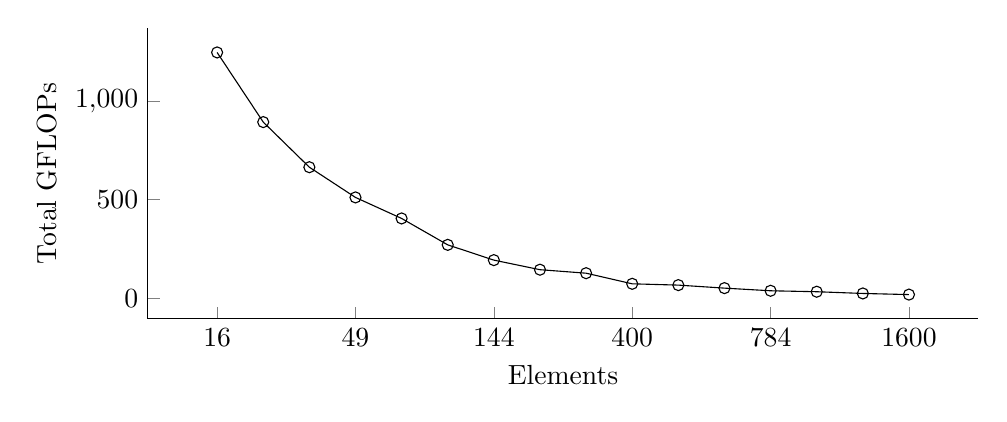
\begin{tikzpicture}
    \begin{axis}[
        height=15em,
        width=\linewidth,
        axis x line*=bottom,
        axis y line*=left,
        symbolic x coords = {16, 25, 36, 49, 64, 100, 144, 196, 225, 400, 441, 576, 784, 900, 1225, 1600},
        xtick = {16, 49, 144, 400, 784, 1600},
        ytick = {0, 500, 1000, 1500},
        domain = 16:1600,
        range = 0:1500,
        xlabel={Elements},
        ylabel={Total GFLOPs}]
        \addplot[
            mark=o,
            color=black] coordinates {
            	(16, 1244.6784)
            	(25, 892.1854771)
            	(36, 663.82848)
            	(49, 510.93504)
            	(64, 404.52048)
            	(100, 270.8420198)
            	(144, 193.61664)             	 
            	(196, 145.152) 
            	(225, 127.4550682) 
            	(400, 73.68496128) 
            	(441, 67.09248) 
            	(576, 51.8616) 
            	(784, 38.46528) 
            	(900, 33.63397632) 
            	(1225, 24.89647104)
            	(1600, 19.16804736)		
            };
    \end{axis}
\end{tikzpicture}

            
